		\documentclass{report}
		
		% Info
		\title{Cinematic storytelling in VR}
		\author{Wouter Vanmulken}
		\date{December 2017}
		
		% Packages 
		\usepackage{graphicx}
		\usepackage{hyperref}
		
		%Titles
		\usepackage[T1]{fontenc}
		\usepackage{titlesec, blindtext, color}

		\definecolor{gray75}{gray}{0.75}
		\newcommand{\hsp}{\hspace{20pt}}
		\titleformat{\chapter}[hang]{\Huge\bfseries}{\thechapter\hsp\textcolor{gray75}{|}\hsp}{0pt}{\Huge\bfseries}
		\setlength{\parindent}{0em}
		\setlength{\parskip}{1em}
		\usepackage[a4paper, total={6in, 8in}]{geometry}
		\usepackage[scaled]{helvet}
		\renewcommand\familydefault{\sfdefault} 
		\usepackage[T1]{fontenc}
		
		\usepackage{todonotes}
		\usepackage{gensymb}
		\usepackage{graphicx}
		\usepackage{float}
		\usepackage{url}
		
		\usepackage{apacite}
		\bibliographystyle{apacite}

		
		\begin{document}
			
				\pagenumbering{gobble}
				\maketitle
				\tableofcontents
				\newpage
				\pagenumbering{arabic}
		
				\chapter{Introduction}
				
				This is a research paper about storytelling in VR. As there is still a lot of information undiscovered about storytelling in VR, i will also be talking about my personal observations on VR storytelling experiences. Because this is a fairly new domain it can be quite hard to get true scientific research. And therefore most of the solutions to problems being discussed in this research document and are subject to change as we explore more of the domain.
				
				\chapter{Research questions}
		
				To be able to research the subject of Cinematic storytelling in VR, i made three questions to guide me through the process.
				\begin{itemize}
					\item How can we make people feel present in a story?
					\item How can we keep people from missing key story details?
					\item How can we grab the attention of a user?
				\end{itemize}

				My first intention of this research was to find how cinematic composition translates in VR. But composition in VR has a lot more aspects than just how a single image looks like. A VR storytelling experience is more like a play than a film. And therefore i will look into how to get the users attention ,keeping it and if we even want to focus it at all.
				

				
				\chapter{How can we make people feel present in a story ?}
				
				\section{Resources}	
				Making people feel present is a delicate balance, a world that doesn't feel right can be a big problem in a storytelling experience. A real-world example of this would be, someone talking during a film. This often brings people back to reality and can be quite frustrating. Although this might be annoying when watching a film, it can be quite devastating while in VR. Breaking the illusion of a virtual world even once can make it feel unreal or even more important, uninteresting.

				Currently there isn't a lot of official research on what these things might be in relation to cinematic experiences. But luckily there still is Oculus story studio. Story studio was a department of Oculus specifically set up to test how cinematic experiences in VR can be created. To research the subject they took the first steps into animating storytelling experiences. With the motto of "story is king", they are currently still \textbf{the} resource on storytelling in VR. 
				
				Unfortunately the department has been closed since they didn't want to compete in a marketplace they were creating research for. But not before they put a lot of the research online on their blog and making some amazing proof-of-concept pieces like Henry and Dear Angelica. Currently they are still the most valuable resources about storytelling in VR.
				
				The only way to really solve these problem is to make experiences. So i'm glad that there are companies like \href{http://www.penrosestudios.com/}{Penrose studios}, \href{http://www.baobabstudios.com/}{Baobab studios} and \href{https://with.in/}{Within} to take over the torch.

				%https://www.oculus.com/story-studio/blog/5-lessons-learned-while-making-lost/
				\section{Routine}\label{chap:Routine}
				
				When you go to a film you start by buying a ticket then you maybe go buy some popcorn or some other snack. And after that you usually still have another 5 minutes of sitting there or some commercials. You mentally prepare yourself during this time and get in a different mindspace. This can be quite crucial in VR. Since we don't have a ticketbooth or popcorn stand. You're just instantly dropped into a new environment. 
				
				This often leads to people feeling overwhelmed and stop paying attention. There is so much to see that your story might not be that interesting compared to the environment. Therefore we need to give the users some time before actually starting the story. In this time they can acclimate to the environment and look around at the interesting world you created.
				
				To make such a routine you could use three phases.
				
				\subsection{Introduction}
				In this phase there shouldn't be much in the users environment. In Lost story studio used a black room with "fi the firefly". This phase is mostly designed for users who haven't had a lot of VR experience and are often overwhelmed the first time they are. So there is a dark room where a firefly flies and react around you. This way there is an introduction to a different world and how it reacts to you. It can also be a good palette cleanser since it starts in entirely black environment with only one point of interest. This is usually a good distraction from the real world and a introduction to the virtual one.
				
				\subsection{Acclimating to the environment}
				In this phase the user gets put into the actual environment, and let the user look around a bit. At this point users might be overwhelmed with the world you created and look around a bit exploring all the different objects and maybe some sound. This phase should take about 40-50 seconds according to story studio\todo{reference maybe ?}. Be sure not to have \textbf{any} key story details during this phase and let the user truly experience what it's like to be present in your world.
				
				\subsection{Starting the story}
				Now that the users is acclimated and has seen enough of the environment they are ready to listen to your story. To begin the story it might be a good idea to play some sound to set the mood and let them know things are about to start. In the meanwhile you can add your opening credits to the scene making them aware that the story will begin shorty as well as that they have to look to a specific direction. But even now people might still be fascinated by the environment or simply looking the other direction. To avoid this a bird flies by in the beginning of Lost, which flies towards the opening credits and makes the user focus on the important part of you scene.
				
				\subsection{Actual Story}
				Now that your user has settled in and knows which direction to look at, you can start actually telling your story.

				
				\section{Common issues}
				
				% https://www.oculus.com/story-studio/blog/the-swayze-effect/
				\subsection{The Swayze effect}
				Accurately named after actor Patrick Swayze from the film ghost. This is an effect where the user isn't acknowledged in the world.
				
				There is often a lot to look at in a VR world which can often lead people to be distracted in your experience which might not be all to great for your story. To get peoples attention they should be interested in the characters that are in the story. One of the most important part of this is to acknowledge the user. We feel left out when we're not acknowledged and don' feel for or are uninterested in the characters. Thus you need to acknowledge people in your world. In Henry, he actually looks at you, this acknowledgement is kind of key. And even though it doesn't really make sense that he looks at you because you don't actually exist in the story, it makes Henry feel real.
				
				So to make sure that your audience is more interested in the story than your surroundings you need to acknowledge them to make a character feel more real and interesting.
				
				If you wish to learn more about this effect you can do so  \href{https://www.oculus.com/story-studio/blog/the-swayze-effect/}{here}.
				
				% https://www.oculus.com/story-studio/blog/5-lessons-learned-while-making-lost/ 4 Be aware of Spatial Story Density
				\subsection{Spatial Story Density}
				\textit{``If only one thing happens in VR at any given time, as is the case in film, the world quickly starts to feel empty and strangely fake.''} - Saschka Unseld (Oculus Story studio)

				This quote explains quite well what section is about. Basically when you're in a room you might not immediately notice smaller details like pictures hanging on a wall or things that might represent the characters. These things can and should be intermittently noticed by the viewer to enchance the characters. If things like these are absent we might as well have used a black room to show you the story. 				
				It's important to have these kind of things because people sometimes drift off and look and feel around the room. And when they are absent it can like Saschka Unseld said feel empty or fake.
				
				% https://www.oculus.com/story-studio/blog/the-problem-with-reality/
				\subsection{Working space and the real world}
				In VR walking into objects can be quite jarring and even world-breaking. Such it should be avoided at all cost. Unfortunately it can be quite hard to do this in a cinematic experience. Because you are mostly confined to one space in a cinematic experience you need to be in a ideal position in your movement-space. 
				Figure\ref{fig:area_most} displays the ideal starting position of the user, in this case you have the ideal world-space to movement-space. You spawn in to the scene in the middle and walk everywhere in you movement-space. Figure \ref{fig:area_least} is a somewhat more likely case of what happens when you spawn into the experience. The movement-space and world-space don't match causing things to be off and might enable the user to walk into things or restrict them from experiencing certain parts of the experience. Therefore you need to be careful with where you spawn the user as well as putting things closer or farther from the movement-space. \todo{paragraphing and structuring}
				
				\begin{figure}[!h]
					\centering
					\begin{minipage}[b!]{0.35\textwidth}
						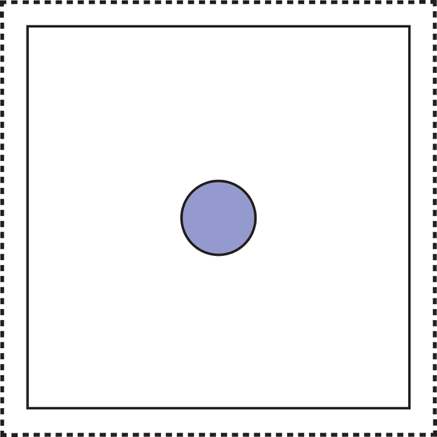
\includegraphics[width=\textwidth]{img/area_most.png}
						\caption{Best case scenario.}
						\label{fig:area_most}
					\end{minipage}
					\hfill
					\begin{minipage}[b!]{0.4\textwidth}
						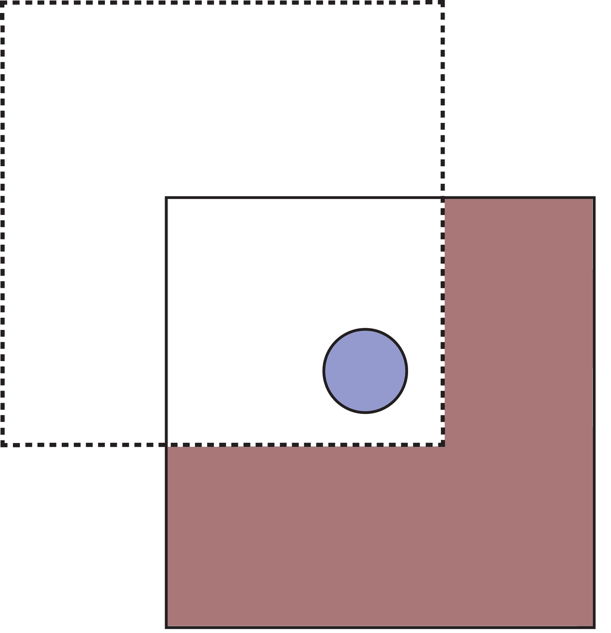
\includegraphics[width=\textwidth]{img/area_least.png}
						\caption{Worst case scenario.}
						\label{fig:area_least}
					\end{minipage}
				\end{figure} \todo{might want to rewrite this}
			
				After looking into the spacing of movement- to world-space you still have one problem. And that is going from scene to scene without spawning into objects. You can somewhat control where your user spawns but if you have some kind of objects in the world-space and they spawn into it, it might be quite jarring. Figure \ref{fig:area_object} is an excellent visualisation of this. 
				
				\begin{figure}[h!]
					\centering
					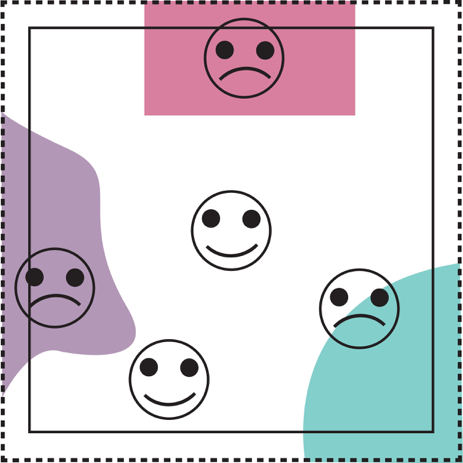
\includegraphics[width=\linewidth/2]{img/area_in_object.png}
					\caption{Spawning into objects.} 
					\label{fig:area_object}
				\end{figure}
				
				\chapter{How can we keep people from miss key story details ?}
				
				You probably noticed that the title of this chapter is missing an "ing". This is just an example of how a users would feel, missing a part of the story in VR. Missing information can get quite frustrating as you can imagine, in this instance you probably blamed me and you would be right to do so. In a VR experience the same thing would happen. The user thinks your experience is poorly made and start to doubt the world as well as feel stupid that they didn't notice the information.
				
				\section{Letting go}
				
				
				\section{Guiding attention}
				
				
				
				\todo{write the chapter}
				
				\chapter{How can we grab the attention of a user ?}
				
				\begin{figure}[h!]
					\centering
					
\includegraphics[width=\linewidth/3]{img/pow.jpg}
					\caption{Attention grabbing example.}
					\label{fig:pow}
				\end{figure}
				
				\section{Should we be guiding the users focus}
				Before we can even answer the question of how we can grab the attention we need to answer the question of if we should. VR gives us 360$^{\circ}$ vision of a alternate reality, so should we limit ourselves because we aren't used to it yet. When the first film was projected, which was of a train coming into the station, people wanted to jump out of their seats \todo{add source "der spiegel" for this} but with time we've overcome this. These days 3D films don't even make us flinch when something is coming at you. The same thing happens when people enters VR for the first time. If you fire a projectile at them, they will move away from it and if you make them fall they'll try to cushion their impact by bending their knees. Currently we are still in the stage were people keep jumping out in front of the train. But looking at how cinema progressed, VR might as well. 
				
				So keeping this example in mind, should we be catering purely to people who want to jump away from the train or should we be finding new ways to make people comfortable with standing in front of that train.
				
				\section{Limiting attention space to 180$^{\circ}$}
				The team that made Henry said in a presentation that this is  still a big problem, and one that they currently don't have a solution for. They found that for now they were still doing experiences in 180 degrees and would in the future like to find a better solution to this. Which they partly did in Dear angelica wherein they used 360 degree of the users environment to draw what can only be described as a VR comic book being drawn while you look. In my opinion this had still a major disadvantage and that it lost me a couple of times. Which made me feel like a absolute idiot and like i was missing a part of the story, which frustrated me endlessly. That being said it was an amazing experiment in 360$^{\circ}$ is storytelling.
				
				\section{Tools to use}
			
				Now that we have looked at what things we might and might not want to do, we can look at tools that can be used to focus a users attention.
				
				
				%phantom sound https://www.oculus.com/story-studio/blog/binaural-audio-for-narrative-vr/
				\subsection{Binaural audio}
				Binaural audio is one of the most intrusive as well as effective tools in your toolbox. Which is probably also why its the first one everyone comes up with. It's effective because we see sudden and unexpected sound as something to investigate. This would've been a huge advantage when there were still a lot of dangers in the world, but now we can use it to catch someone's attention.
				
				This also means that we need a source of that sound to make sure it's not a threat. If you make a sound and don't explain it, people will get uncomfortable. During the making of Henry, Story studio wanted to incorporate music. But because this is a VR experience we're talking about they wanted to make it spatial audio. And what they found was that when they put the different sound sources into the scene while it was black the users where fine with it. But when people were put into a scene that had no visible sound sources but still sound coming from that direction, they started to get uncomfortable. So what they did was just use simple stereo audio and they found was that people were already used to having headphones. And were therefore fine with it.
				
				So to use sound properly you basically have to mimic the real world. 
				And make sure to :
				\begin{itemize}
					\item Don't overuse it
					\item Explain your sounds when visible
					\item Use stereo audio for narration and music
				\end{itemize}
				There is still a lot to learn about audio in VR and what we can an cannot use, so sometimes you just have to test what works best for your experience. 
				
				
				\subsection{Pattern interrupt and negative space}
				You've probably seen enough images like figure \ref{fig:PatternInterrupt}. Our brains are programmed to see patterns, so when a pattern is disrupted it stands out. This also has some similarities with a technique used in film called negative space which can be seen in figure \ref{fig:NegativeSpace}. This uses a lot of unused space to make the used space that more important. 
							
				
				\begin{figure}[!h]
					\centering
					\begin{minipage}[b!]{0.35\textwidth}
						\includegraphics[width=\textwidth]{img/PatternInterrupt.jpg}
						\caption{Pattern interrupt.}
						\label{fig:PatternInterrupt}
					\end{minipage}
					\hfill
					\begin{minipage}[b!]{0.4\textwidth}
						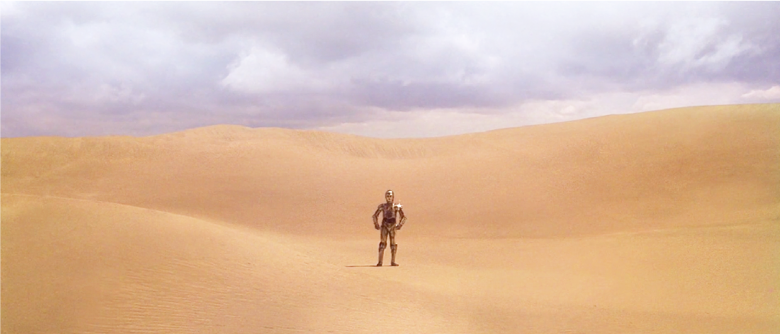
\includegraphics[width=\textwidth]{img/C3PONegativeSpace.png}
						\caption{Negative space.}
						\label{fig:NegativeSpace}
					\end{minipage}
				\end{figure}
				
				This technique also works in VR and is actually used in the intro of Henry.\todo{reference}.	By making everything but the subject equal or in a pattern, we can still grab peoples attention. \todo{improve or remove this}				
				\todo{warning about how to use it}				
				In figure \ref{fig:henryIntro} we can see how negative space is used in the intro of henry. They have a intro where you can sit down, some music starts playing and then slowly after the title card is displayed a story is told by a narrator and picture frames pop up to enhance the experience. this is an excellent use of negative space because it isn't used to focus your attention full time but rather to guide you to the starting point. People need a kind of pallet cleanser before going into such an experience as talked about in \autoref{chap:Routine}.\todo{make sure to finish this}
				
				\todo{fix the henry image formatting}
				\begin{figure}[h!]
					\centering
					 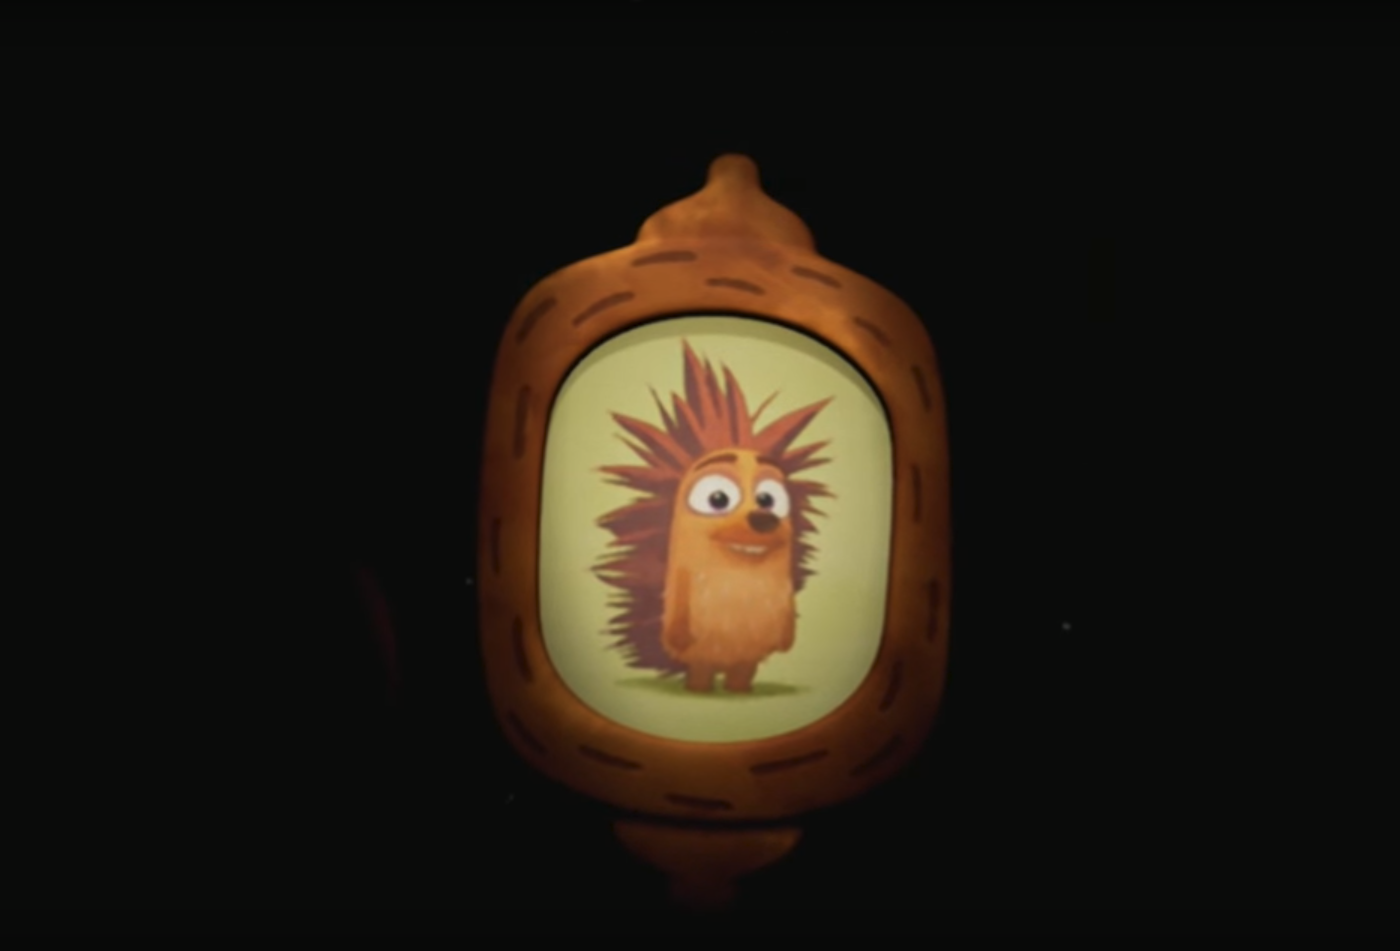
\includegraphics[width=30em]{img/henry_intro.png}
					\caption{Intro of Henry.}
					\label{fig:henryIntro}
				\end{figure}
				\subsection{Guiding the attention} \todo{reread and adjust !!!!}
				
				Once you have the attention you have to keep it. This can be done by guiding the gaze. Dear angelica is an excellent example of this, it uses writing to grab and guide your attention. This way the user knows where to look but isn't limited to it. This is also one of the most important realisations to have as a director of a storytelling experience. Know that your audience might not be following your gaze!
				
				This means that you can try and try to have every moment of your environment be focused on your story, but still fail in achieving it in your viewers. Users can be quite different and might hang on to previous story points or may just simply be amazed by their surroundings. This is a key point of storytelling in VR.
				
				You can't completely focus all of you attention on one point. Now you might think, what if i make only one thing happen at a time. Surely the user will focus on the one thing that is interesting. Unfortunately this will make the world feel fake\todo{add citation of blog}. When only one thing around us is making noise or is interesting the entire world seems fake because the real world isn't like that. When people are put into sensory deprivation tanks the often begin to hallucinate because the brain needs input. Now of course people won't start hallucinating in VR because there still is a lot of input but if there is only one thing to focus on or happening at a particular time the world seems fake. 
				This has primarily to do with sound. Listen to what's around you right now and notice how there is sound coming from all directions. May it be the water running through the radiator, a clock gently ticking or cars driving by. Our brains filter out a lot of uninteresting noise, but when it isn't there the brain starts to notice.
				
								
				\chapter{Conclusion}
				\section{Where is VR storytelling currently}
				
				Currently there are two real options for VR storytelling, 3D video and animation. In this research paper i didn't really go into 3D video as i don't really see it as a good option right now. The resolution is still to low and it often still relies on movement which can be quite nauseating in VR. 
				
				At this point in time there is still a lot of research to be done in the field. As well as making cinematic VR experiences becoming more common place. If you think about VR you don' t immediately think about films. Even i had a hard time finding other experiences then Henry which needs to change. At this point in time cinema in VR is a long way from being common place which is quite a shame.
				
				
				
				\section{Personal opinion}
				
				Making cinematic VR experiences is hard. The field is still very young and there isn't really a real blueprint yet. To get cinema in VR off the ground a lot of research needs to be done as well as just making experiences and find what we can learn from them. To fully understand the medium we need to start making mistakes so we can learn from them.
				But there will come a point in time were cinematic experiences will be common place and might even replace film.

				
				\section{The future of VR storytelling}
				
				There are multiple companies to that are starting to see the real value of VR as a new medium for film, and they are all doing interesting and new things. Unfortunately there is still a lot unknown about the space and can be hard to get into.
				 				
				There is definitely a place for storytelling in VR and big one as well. And new experiences are making it more and more of a reality. Research is still hard to come by and can only truly be done by making new experiences. So even though there is still a long road ahead, it's one we have to walk to find out where it leads.
				
				\chapter{Sources}
				
				\section{Images}
				
				
				image pattern interrupt :\ref{fig:PatternInterrupt} \href{https://dealerwebb.com/WebSites/1626/Images/Blogs/2241/PatternInterrupt.jpg}{https://dealerwebb.com/WebSites/1626/Images/Blogs/2241/PatternInterrupt.jpg}
				
				star wars negative space :\ref{fig:NegativeSpace} \href{https://venngage-wordpress.s3.amazonaws.com/uploads/2015/12/negative-space.png}{https://venngage-wordpress.s3.amazonaws.com/uploads/2015/12/negative-space.png}
				
				Henry intro : \ref{fig:henryIntro} \href{https://youtu.be/IUY2yI5F16U}{https://youtu.be/IUY2yI5F16U}
				
				Pow attention image :\ref{fig:pow}
				\href{http://moziru.com/images/pop-art-clipart-pow-12.jpg}{http://moziru.com/images/pop-art-clipart-pow-12.jpg}
				
				\section{Literature}
				
				\bibliography{bib}
				
		\end{document}